\documentclass{article}
\usepackage{graphicx}
\usepackage{float}
\usepackage{amsmath}

\title{CTA200 Assignment 3}
\author{Wendy Tso}
\date{May 2026}

\begin{document}

\maketitle

\section{Introduction}
This assignment studies two nonlinear dynamical systems: the Mandelbrot set and the Lorenz system. Both systems demonstrate how simple deterministic rules can generate complex and chaotic behavior.

\section{Question 1: Mandelbrot Set}

The Mandelbrot set is defined by iterating the complex recurrence relation
\[
z_{n+1} = z_n^2 + c,
\]
where $c = x + iy$ is a complex parameter and $z_0 = 0$.

For each point $c$ in the complex plane, we determine whether the sequence remains bounded or diverges. Points that remain bounded are classified as part of the Mandelbrot set.

Two visualizations are produced:
(i) a binary plot showing bounded vs divergent points, and  
(ii) an escape-time plot showing the iteration at which divergence occurs.

\section{Question 2: Lorenz System}

The Lorenz system is given by:
\[
\dot X = -\sigma(X-Y), \quad
\dot Y = rX - Y - XZ, \quad
\dot Z = -bZ + XY.
\]

We numerically solve this system using \texttt{solve\_ivp} with parameters $\sigma = 10$, $r = 28$, and $b = 8/3$. The system is known to exhibit chaotic dynamics and strong sensitivity to initial conditions.

\newpage

\section*{Results: Question 1}

\begin{figure}[H]
\centering
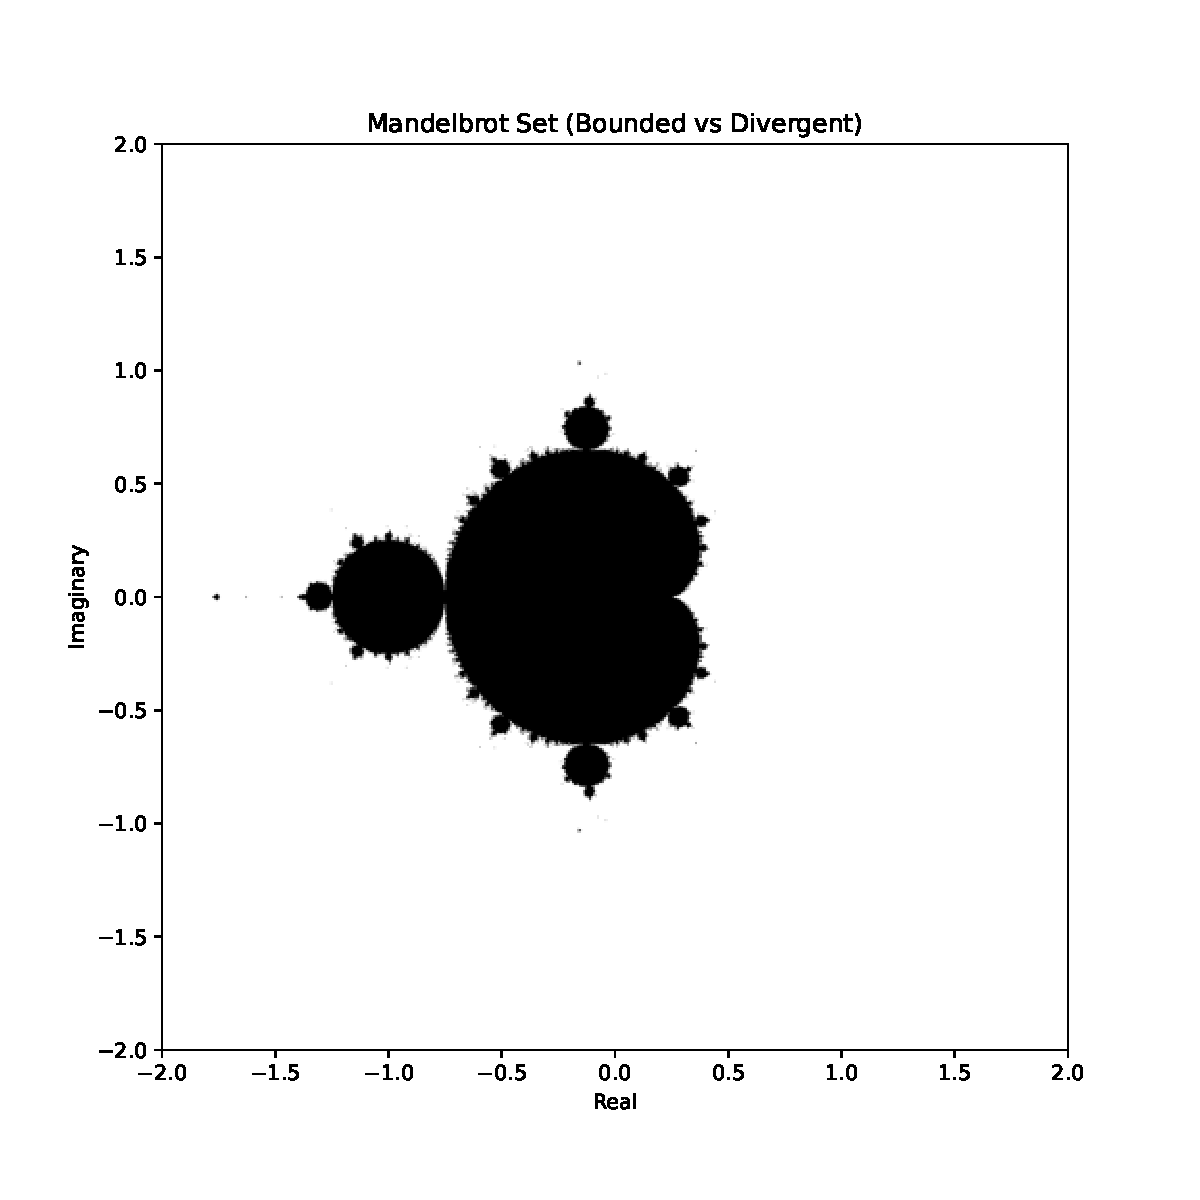
\includegraphics[width=0.8\textwidth]{Mandelbrot_bounded_divergent.pdf}
\caption{Mandelbrot set: bounded vs divergent points.}
\end{figure}

\begin{figure}[H]
\centering
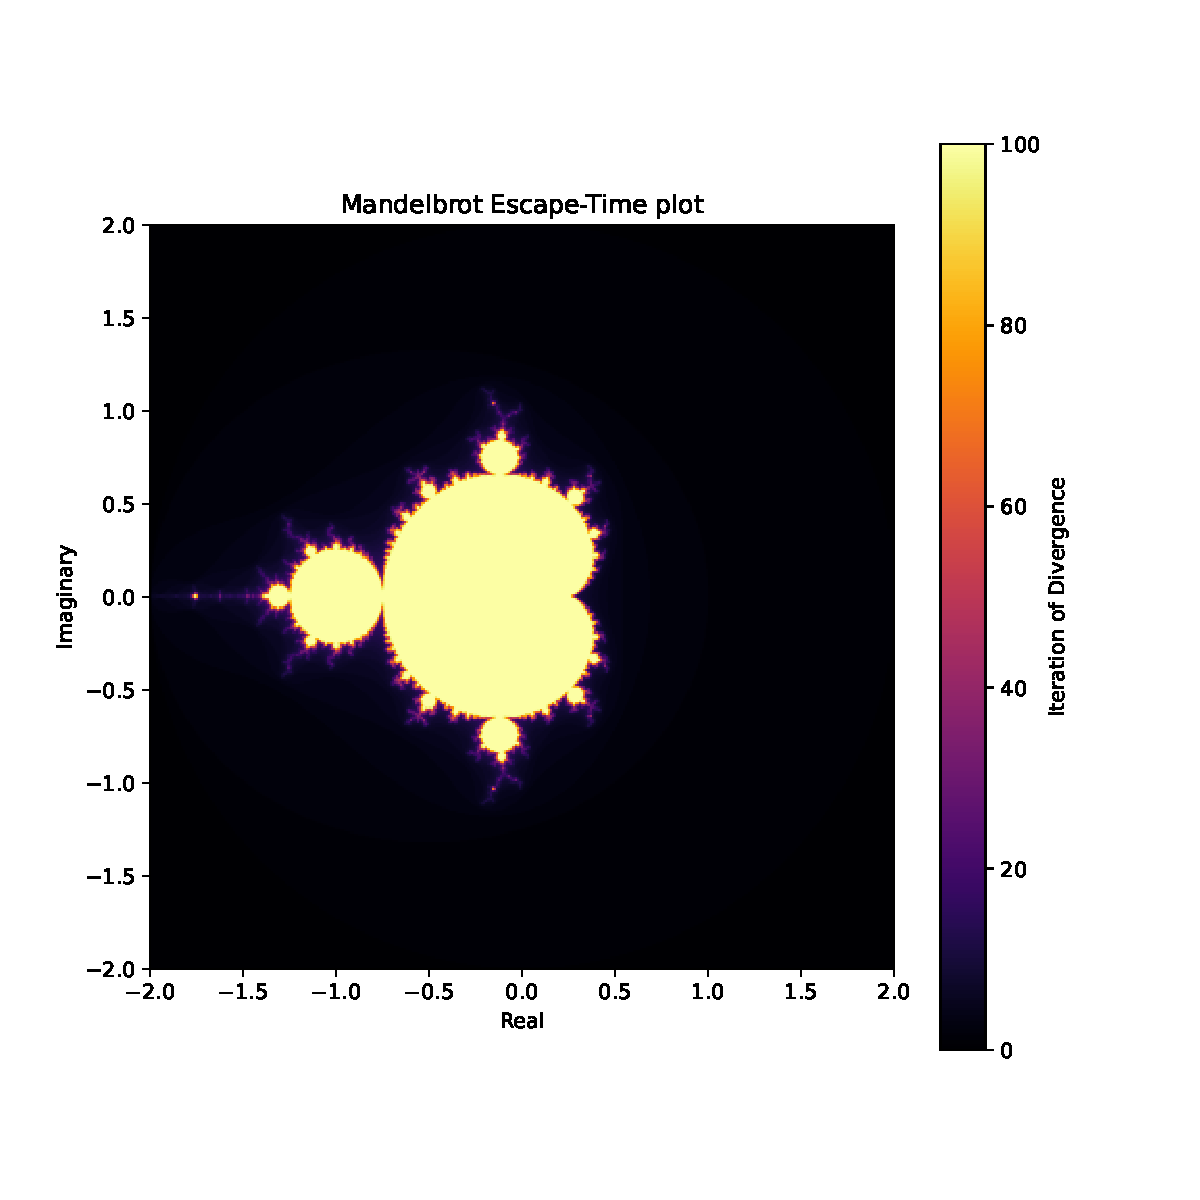
\includegraphics[width=0.8\textwidth]{Mandelbrot_escape_time.pdf}
\caption{Mandelbrot escape-time plot.}
\end{figure}

\newpage

\section*{Results: Question 2}

\begin{figure}[H]
\centering
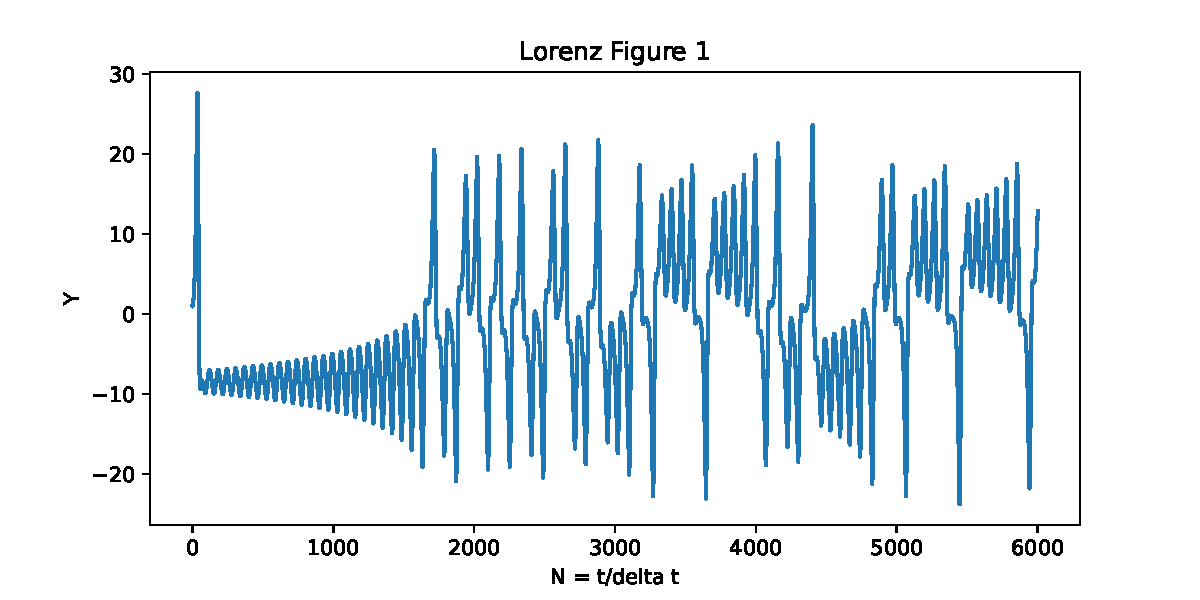
\includegraphics[width=0.85\textwidth]{lorenz_fig1.pdf}
\caption{Time evolution of the Lorenz system (variable $Y$).}
\end{figure}

\begin{figure}[H]
\centering
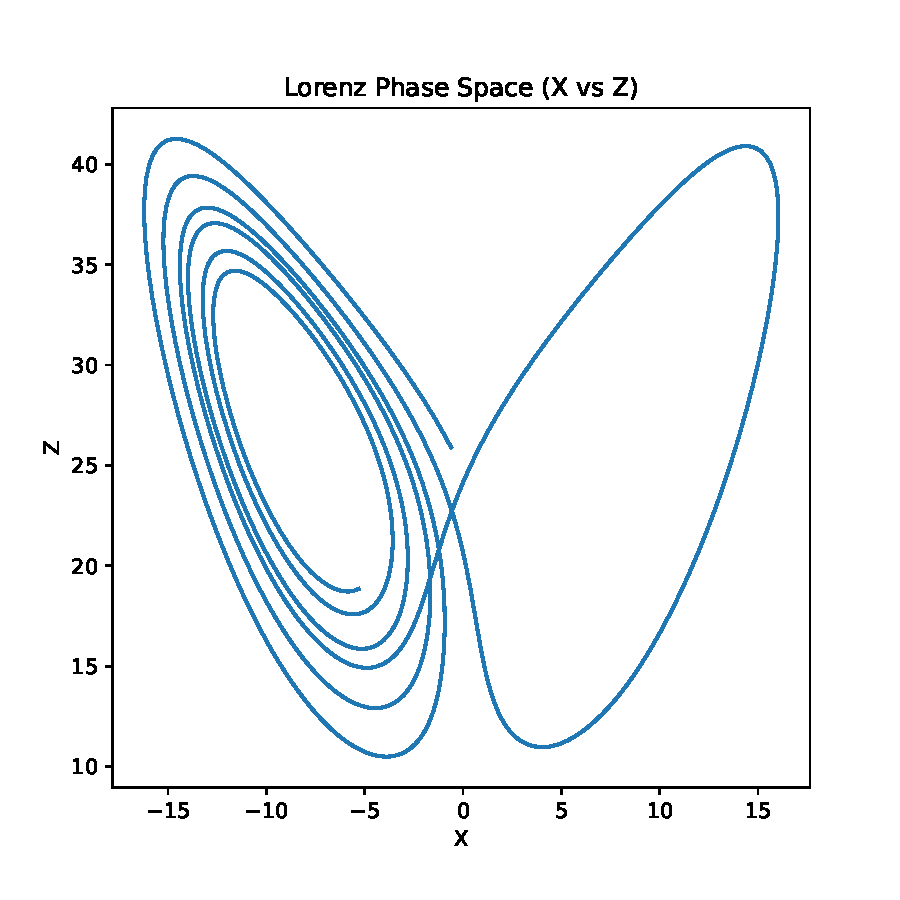
\includegraphics[width=0.75\textwidth]{lorenz_fig_xz.pdf}
\caption{Lorenz phase space projection ($X$ vs $Z$).}
\end{figure}

\begin{figure}[H]
\centering
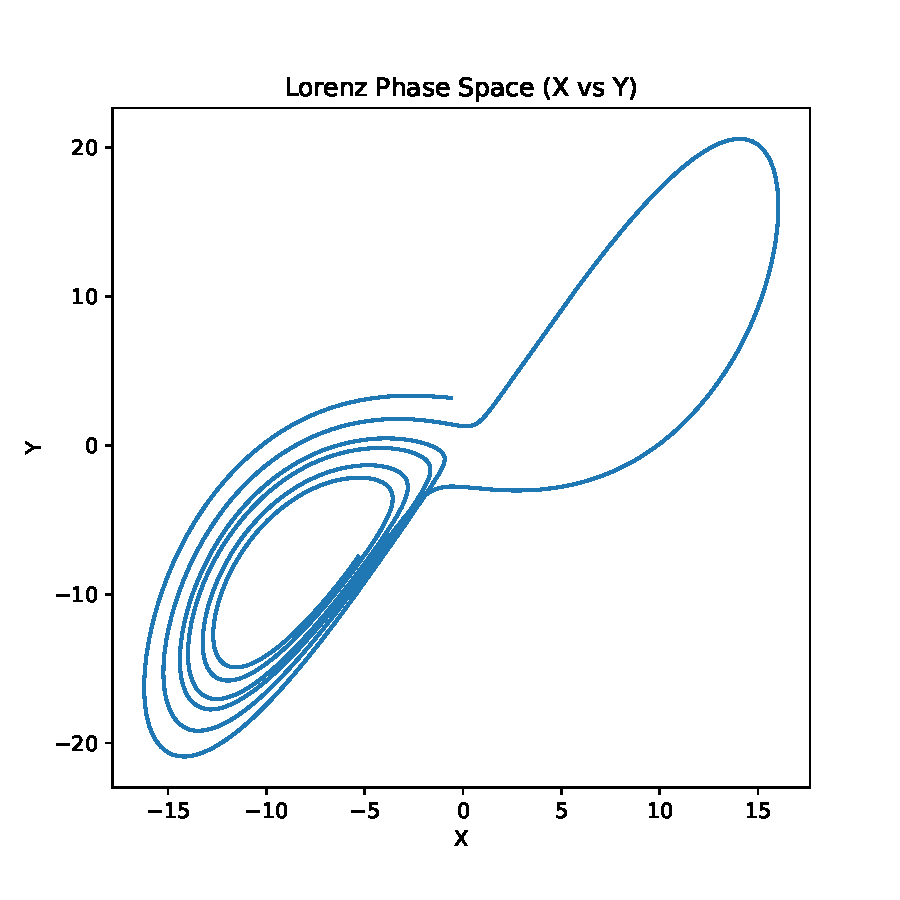
\includegraphics[width=0.75\textwidth]{lorenz_fig_xy.pdf}
\caption{Lorenz phase space projection ($X$ vs $Y$).}
\end{figure}

\begin{figure}[H]
\centering
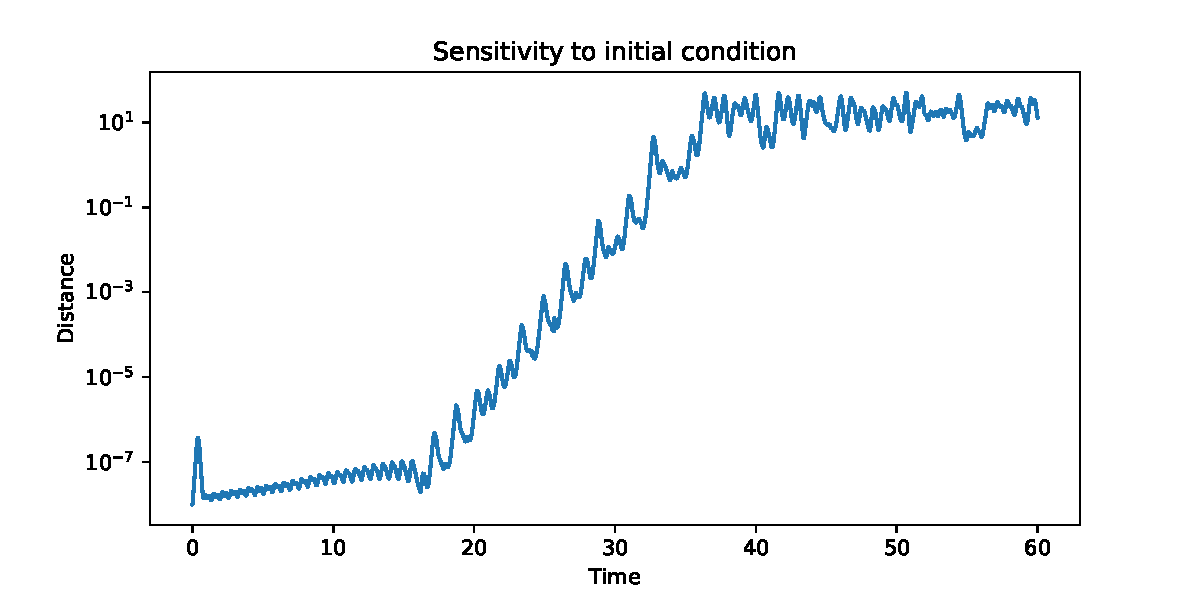
\includegraphics[width=0.85\textwidth]{sensitivity_initial_condition.pdf}
\caption{Sensitivity to initial conditions showing exponential divergence.}
\end{figure}

\end{document}
